\documentclass[11pt]{article}
\usepackage[margin=1in]{geometry}
\usepackage{amsmath,amssymb,booktabs,array,longtable}
\usepackage{graphicx}
\graphicspath{{figures/}}
\usepackage{hyperref}
\usepackage{enumitem}
\usepackage{titlesec}
\usepackage{float}
\usepackage{caption}
\usepackage{mathtools}
\usepackage{setspace}

\onehalfspacing

\begin{document}

\begin{center}
{\LARGE\textbf{Shiv Nadar University Chennai}}\\[4mm]
\end{center}

\renewcommand{\arraystretch}{1.6}
\setlength{\tabcolsep}{10pt}

\begin{center}
\begin{tabular}{|p{4cm}|p{9.5cm}|}
\hline
\textbf{Degree \& Branch} & B.Tech Artificial Intelligence \& Data Science, Semester V \\ \hline
\textbf{Subject} & CS3807 -- Deep Learning Laboratory \\ \hline
\textbf{Name} & Madhav.S \\ \hline
\textbf{Section} & AIDS `B' \\ \hline
\textbf{Register Number} & 24011101066 \\ \hline
\end{tabular}
\end{center}

\vspace{5mm}

\begin{center}
{\Large\textbf{Experiment 3}}\\[1mm]
{\large\textbf{Design and Implementation of a Convolutional Neural Network for Image Classification on CIFAR-10}}
\end{center}

\vspace{4mm}

%----------------------------------------------------------

\section*{1. Objective}

The goal of this experiment is to design, implement, train, and evaluate a Convolutional Neural Network (CNN) using TensorFlow/Keras for multi-class image classification. The experiment aims to build familiarity with the core building blocks of a CNN -- convolution, activation, pooling, flattening, and fully connected layers -- understand how kernels extract visual features, study the effect of key hyperparameters on performance, and evaluate the trained model on a real-world image dataset using standard classification metrics.

%----------------------------------------------------------

\section*{2. Background Theory}

A \textbf{Convolutional Neural Network} is a class of deep learning architecture specifically suited to grid-structured data such as images. Unlike a fully connected network, where every neuron in one layer connects to every neuron in the next, a CNN uses small, learnable filters (kernels) that slide across the image, looking for the same local pattern -- an edge, a corner, a texture -- everywhere in the image at once. This weight sharing is what makes CNNs both far more parameter-efficient and far better suited to images than plain multilayer perceptrons.

\subsection*{Convolution Operation}

For an input feature map $X$ and a kernel $W$ of size $k \times k$, the convolution output at position $(i,j)$ is:

\[
Z(i,j) = \sum_{m=0}^{k-1}\sum_{n=0}^{k-1} W(m,n)\, X(i+m,\, j+n) + b
\]

where $b$ is a bias term shared across the whole feature map produced by that filter. Sliding this small filter across the entire image and repeating it for many different filters is what allows a single convolutional layer to detect many different local patterns simultaneously.

\subsection*{Key Spatial Hyperparameters}

\begin{itemize}
\item \textbf{Kernel size} - how large the receptive field of each filter is (e.g., $3\times3$). Larger kernels see more spatial context per step but cost more parameters and computation.
\item \textbf{Stride} - how many pixels the kernel moves at each step. A stride of 1 preserves detail; a larger stride downsamples faster.
\item \textbf{Padding} - `same' padding keeps the output the same spatial size as the input; `valid' padding shrinks it after every convolution.
\item \textbf{Number of filters} - how many independent feature detectors a layer learns. More filters mean a richer set of learned features, at the cost of more parameters.
\end{itemize}

%----------------------------------------------------------

\section*{3. CNN Building Blocks}

\begin{table}[H]
\centering
\caption{Core CNN Layers and Their Purpose}
\begin{tabular}{p{3.3cm}p{10.5cm}}
\toprule
\textbf{Layer} & \textbf{Purpose} \\
\midrule
Convolutional Layer & Applies learnable kernels that slide over the image to extract local features such as edges, textures, and patterns. \\
Activation (ReLU) & Introduces non-linearity, letting the network model complex, non-linear decision boundaries. \\
Pooling Layer & Downsamples feature maps (Max/Average Pooling), reducing spatial size and computation while keeping the most important activations. \\
Batch Normalization & Normalizes layer activations during training, which stabilizes and speeds up convergence. \\
Flatten Layer & Converts the final 2D feature maps into a 1D vector so it can feed into dense layers. \\
Fully Connected (Dense) Layer & Combines the extracted features to make the final class prediction. \\
Dropout & Randomly deactivates a fraction of neurons during training as a regularizer against overfitting. \\
\bottomrule
\end{tabular}
\end{table}

\textit{Note: this experiment uses only ReLU activations in the hidden layers and Softmax at the output, since the task is 10-way multi-class classification.}

%----------------------------------------------------------

\section*{4. Dataset Description}

\textbf{Dataset:} CIFAR-10\\
\textbf{Source:} Loaded directly via \texttt{tensorflow.keras.datasets.cifar10}\\
\textbf{Link:} \url{https://www.cs.toronto.edu/~kriz/cifar.html}

\begin{table}[H]
\centering
\caption{Dataset Summary}
\begin{tabular}{ll}
\toprule
Total Images & 60,000 ($32\times32$, RGB) \\
Training Images & 50,000 \\
Test Images & 10,000 \\
Classes & 10 (airplane, automobile, bird, cat, deer, dog, frog, horse, ship, truck) \\
Images per Class & 5,000 (perfectly balanced) \\
Missing Values & None \\
Task & Multi-class image classification \\
\bottomrule
\end{tabular}
\end{table}

The class distribution is exactly balanced at 5,000 images per class in the training set, so no class-imbalance handling (oversampling, class weighting, etc.) was needed for this experiment.

%----------------------------------------------------------

\section*{5. Experimental Procedure}

\textbf{Task 1 -- Dataset Exploration:} CIFAR-10 was loaded via the Keras dataset API. Shape, pixel value range, and class distribution were examined before further processing.

\textbf{Task 2 -- Data Preprocessing:} Pixel values were normalized to the $[0,1]$ range, labels were one-hot encoded for the 10 classes, and a 5,000-image validation set was carved out of the training data, leaving 45,000 training images.

\textbf{Task 3 -- Architecture Design:} A CNN with three convolutional blocks (Conv2D + BatchNorm + ReLU + MaxPooling), followed by flattening and two fully connected layers with dropout, was built using the Keras Functional API.

\textbf{Task 4 -- Parameter Analysis:} The trainable parameters of every convolutional layer were computed and manually verified against the formula $(k_h \cdot k_w \cdot c_{in} + 1)\cdot c_{out}$.

\textbf{Task 5 -- Model Training:} The model was trained for 30 epochs with the Adam optimizer, a batch size of 64, real-time data augmentation, and a \texttt{ReduceLROnPlateau} callback to decay the learning rate when validation loss plateaued.

\textbf{Task 6 -- Model Evaluation:} The trained model was evaluated on the held-out 10,000-image test set using accuracy, precision, recall, F1-score, a full classification report, and a confusion matrix.

\textbf{Task 7 -- Feature Map Visualization:} Intermediate activations from every convolutional layer were extracted for a single test image to observe how the network's internal representation changes with depth.

\textbf{Task 8 -- Pooling Strategy Comparison:} A smaller CNN was trained twice, identical except for using Max Pooling vs. Average Pooling, to compare their effect on convergence and accuracy.

\textbf{Task 9 -- Hyperparameter Study:} The same small CNN was trained with two different batch sizes (32 and 128) to observe the effect of batch size on validation accuracy.

%----------------------------------------------------------

\section*{6. Source Code}

The complete implementation, exactly as run in Colab, is hosted on GitHub.

\begin{center}
\url{https://github.com/smadhav2024/Deep_Learning_Lab/tree/main/Lab%203}
\end{center}

The repository contains the full notebook, the requirements needed to run it, and this report's LaTeX source.

%----------------------------------------------------------

\section*{7. Experimental Results}

\subsection*{Dataset Summary}

The dataset was confirmed to have no missing values. After preprocessing, the split produced \textbf{45,000 training images}, \textbf{5,000 validation images}, and \textbf{10,000 test images}, with all 10 classes contributing exactly 5,000 images each to the original training set.

\subsection*{Architecture and Parameter Summary}

\begin{table}[H]
\centering
\caption{Trainable Parameters of Convolutional Layers}
\begin{tabular}{lccc}
\toprule
Layer & Output Shape & Params \\
\midrule
conv1 & $(32,32,32)$ & 896 \\
conv2 & $(32,32,32)$ & 9{,}248 \\
conv3 & $(16,16,64)$ & 18{,}496 \\
conv4 & $(16,16,64)$ & 36{,}928 \\
conv5 & $(8,8,128)$ & 73{,}856 \\
\bottomrule
\end{tabular}
\end{table}

\textbf{Total Convolutional Layer Parameters:} 139,424\\
\textbf{Total Model Parameters (including dense layers and batch norm):} 668,842

A manual check for \texttt{conv1} confirmed the parameter formula: $(3 \times 3 \times 3 + 1) \times 32 = 896$, matching the count reported by Keras exactly.

\subsection*{Training Outcome}

The model was trained for 30 epochs at an initial learning rate of $0.001$, with \texttt{ReduceLROnPlateau} (factor $=0.5$, patience $=3$) monitoring validation loss. The learning rate was reduced three times over the course of training -- at epoch 9 ($0.001 \rightarrow 0.0005$), epoch 16 ($0.0005 \rightarrow 0.00025$), and epoch 28 ($0.00025 \rightarrow 0.000125$) -- each drop coinciding with a validation loss plateau. Training accuracy rose steadily from 77\% to 83\% while validation accuracy fluctuated in the mid-to-high 80s, settling around 84--86\% by the final epochs. A sample of the training log:

\begin{verbatim}
Epoch  1/30 - accuracy: 0.7712 - loss: 0.6598 - val_accuracy: 0.7958 - val_loss: 0.6184
Epoch  5/30 - accuracy: 0.7822 - loss: 0.6311 - val_accuracy: 0.8272 - val_loss: 0.4912
Epoch 10/30 - accuracy: 0.8044 - loss: 0.5682 - val_accuracy: 0.8516 - val_loss: 0.4468
Epoch 15/30 - accuracy: 0.8101 - loss: 0.5470 - val_accuracy: 0.8442 - val_loss: 0.4503
Epoch 20/30 - accuracy: 0.8225 - loss: 0.5129 - val_accuracy: 0.8492 - val_loss: 0.4575
Epoch 25/30 - accuracy: 0.8274 - loss: 0.4990 - val_accuracy: 0.8684 - val_loss: 0.3945
Epoch 30/30 - accuracy: 0.8326 - loss: 0.4867 - val_accuracy: 0.8482 - val_loss: 0.4590
\end{verbatim}

The full epoch-wise log is summarized in Section 9, Performance Tables.

\subsection*{Test Set Evaluation}

\begin{table}[H]
\centering
\caption{Test Set Performance of the CNN (30 epochs, batch size 64)}
\begin{tabular}{lc}
\toprule
Metric & Value \\
\midrule
Test Loss & 0.4376 \\
Accuracy & 0.8527 \\
Precision (weighted) & 0.8553 \\
Recall (weighted) & 0.8527 \\
F1-score (weighted) & 0.8501 \\
\bottomrule
\end{tabular}
\end{table}

\begin{table}[H]
\centering
\caption{Per-Class Classification Report}
\begin{tabular}{lccc}
\toprule
Class & Precision & Recall & F1-score \\
\midrule
airplane   & 0.86 & 0.88 & 0.87 \\
automobile & 0.94 & 0.94 & 0.94 \\
bird       & 0.83 & 0.78 & 0.80 \\
cat        & 0.84 & 0.60 & 0.70 \\
deer       & 0.83 & 0.84 & 0.84 \\
dog        & 0.85 & 0.76 & 0.80 \\
frog       & 0.74 & 0.96 & 0.83 \\
horse      & 0.90 & 0.88 & 0.89 \\
ship       & 0.90 & 0.94 & 0.92 \\
truck      & 0.88 & 0.94 & 0.91 \\
\bottomrule
\end{tabular}
\end{table}

The model performs best on vehicle classes - automobile, ship, and truck all cross 0.90 F1 -- which makes sense, since man-made objects tend to have more consistent shapes and colours across images. The weakest class by far is \textbf{cat}, with recall dropping to 0.60: the model correctly finds cats less than two-thirds of the time. \textbf{Frog} shows the opposite pattern - very high recall (0.96) but noticeably lower precision (0.74) - suggesting the model is somewhat over-predicting the frog class, likely pulling in some of the missed cats and dogs. This cat/dog/frog confusion is a well-known difficulty in CIFAR-10, since these classes share overlapping textures, poses, and backgrounds at $32\times32$ resolution.

\subsection*{Pooling Strategy Comparison}

\begin{table}[H]
\centering
\caption{Max Pooling vs. Average Pooling (small CNN, 10,000-image subset, 8 epochs)}
\begin{tabular}{lcc}
\toprule
Pooling Type & Test Accuracy & Test Loss \\
\midrule
Max Pooling & 0.5548 & 1.2726 \\
Average Pooling & 0.5455 & 1.2983 \\
\bottomrule
\end{tabular}
\end{table}

Under identical, short-training conditions, Max Pooling came out slightly ahead of Average Pooling on both accuracy and loss. This is consistent with the general intuition that Max Pooling tends to preserve the strongest, most discriminative activations in a region, while Average Pooling smooths them out -- a difference that mattered even in this quick, small-scale comparison.

\subsection*{Effect of Batch Size}

\begin{table}[H]
\centering
\caption{Effect of Batch Size on Test Accuracy (small CNN, 10,000-image subset, 8 epochs)}
\begin{tabular}{lc}
\toprule
Batch Size & Test Accuracy \\
\midrule
32  & 0.5906 \\
128 & 0.5460 \\
\bottomrule
\end{tabular}
\end{table}

The smaller batch size of 32 reached a noticeably higher accuracy than 128 within the same 8 epochs. Smaller batches update the weights more often per epoch and introduce more gradient noise, which - especially over a short training run - can help the model explore the loss surface more effectively than the smoother, less frequent updates of larger batches.

%----------------------------------------------------------

\section*{8. Generated Plots with Interpretation}

\begin{figure}[H]
\centering

\includegraphics[width=0.6\textwidth]{class_distribution.pdf}
\caption{Class Distribution in the CIFAR-10 Training Set}
\end{figure}
\textbf{Observation:} All ten classes contain exactly 5,000 images, confirming the dataset is perfectly balanced -- no resampling or class weighting was required before training.

\begin{figure}[H]
\centering

\includegraphics[width=0.85\textwidth]{sample_images.pdf}
\caption{Sample Images -- One per Class}
\end{figure}
\textbf{Observation:} Even at $32\times32$ resolution, most classes are visually distinguishable, though some - particularly cat, dog, and deer - share similar colour properties and poses.

\begin{figure}[H]
\centering
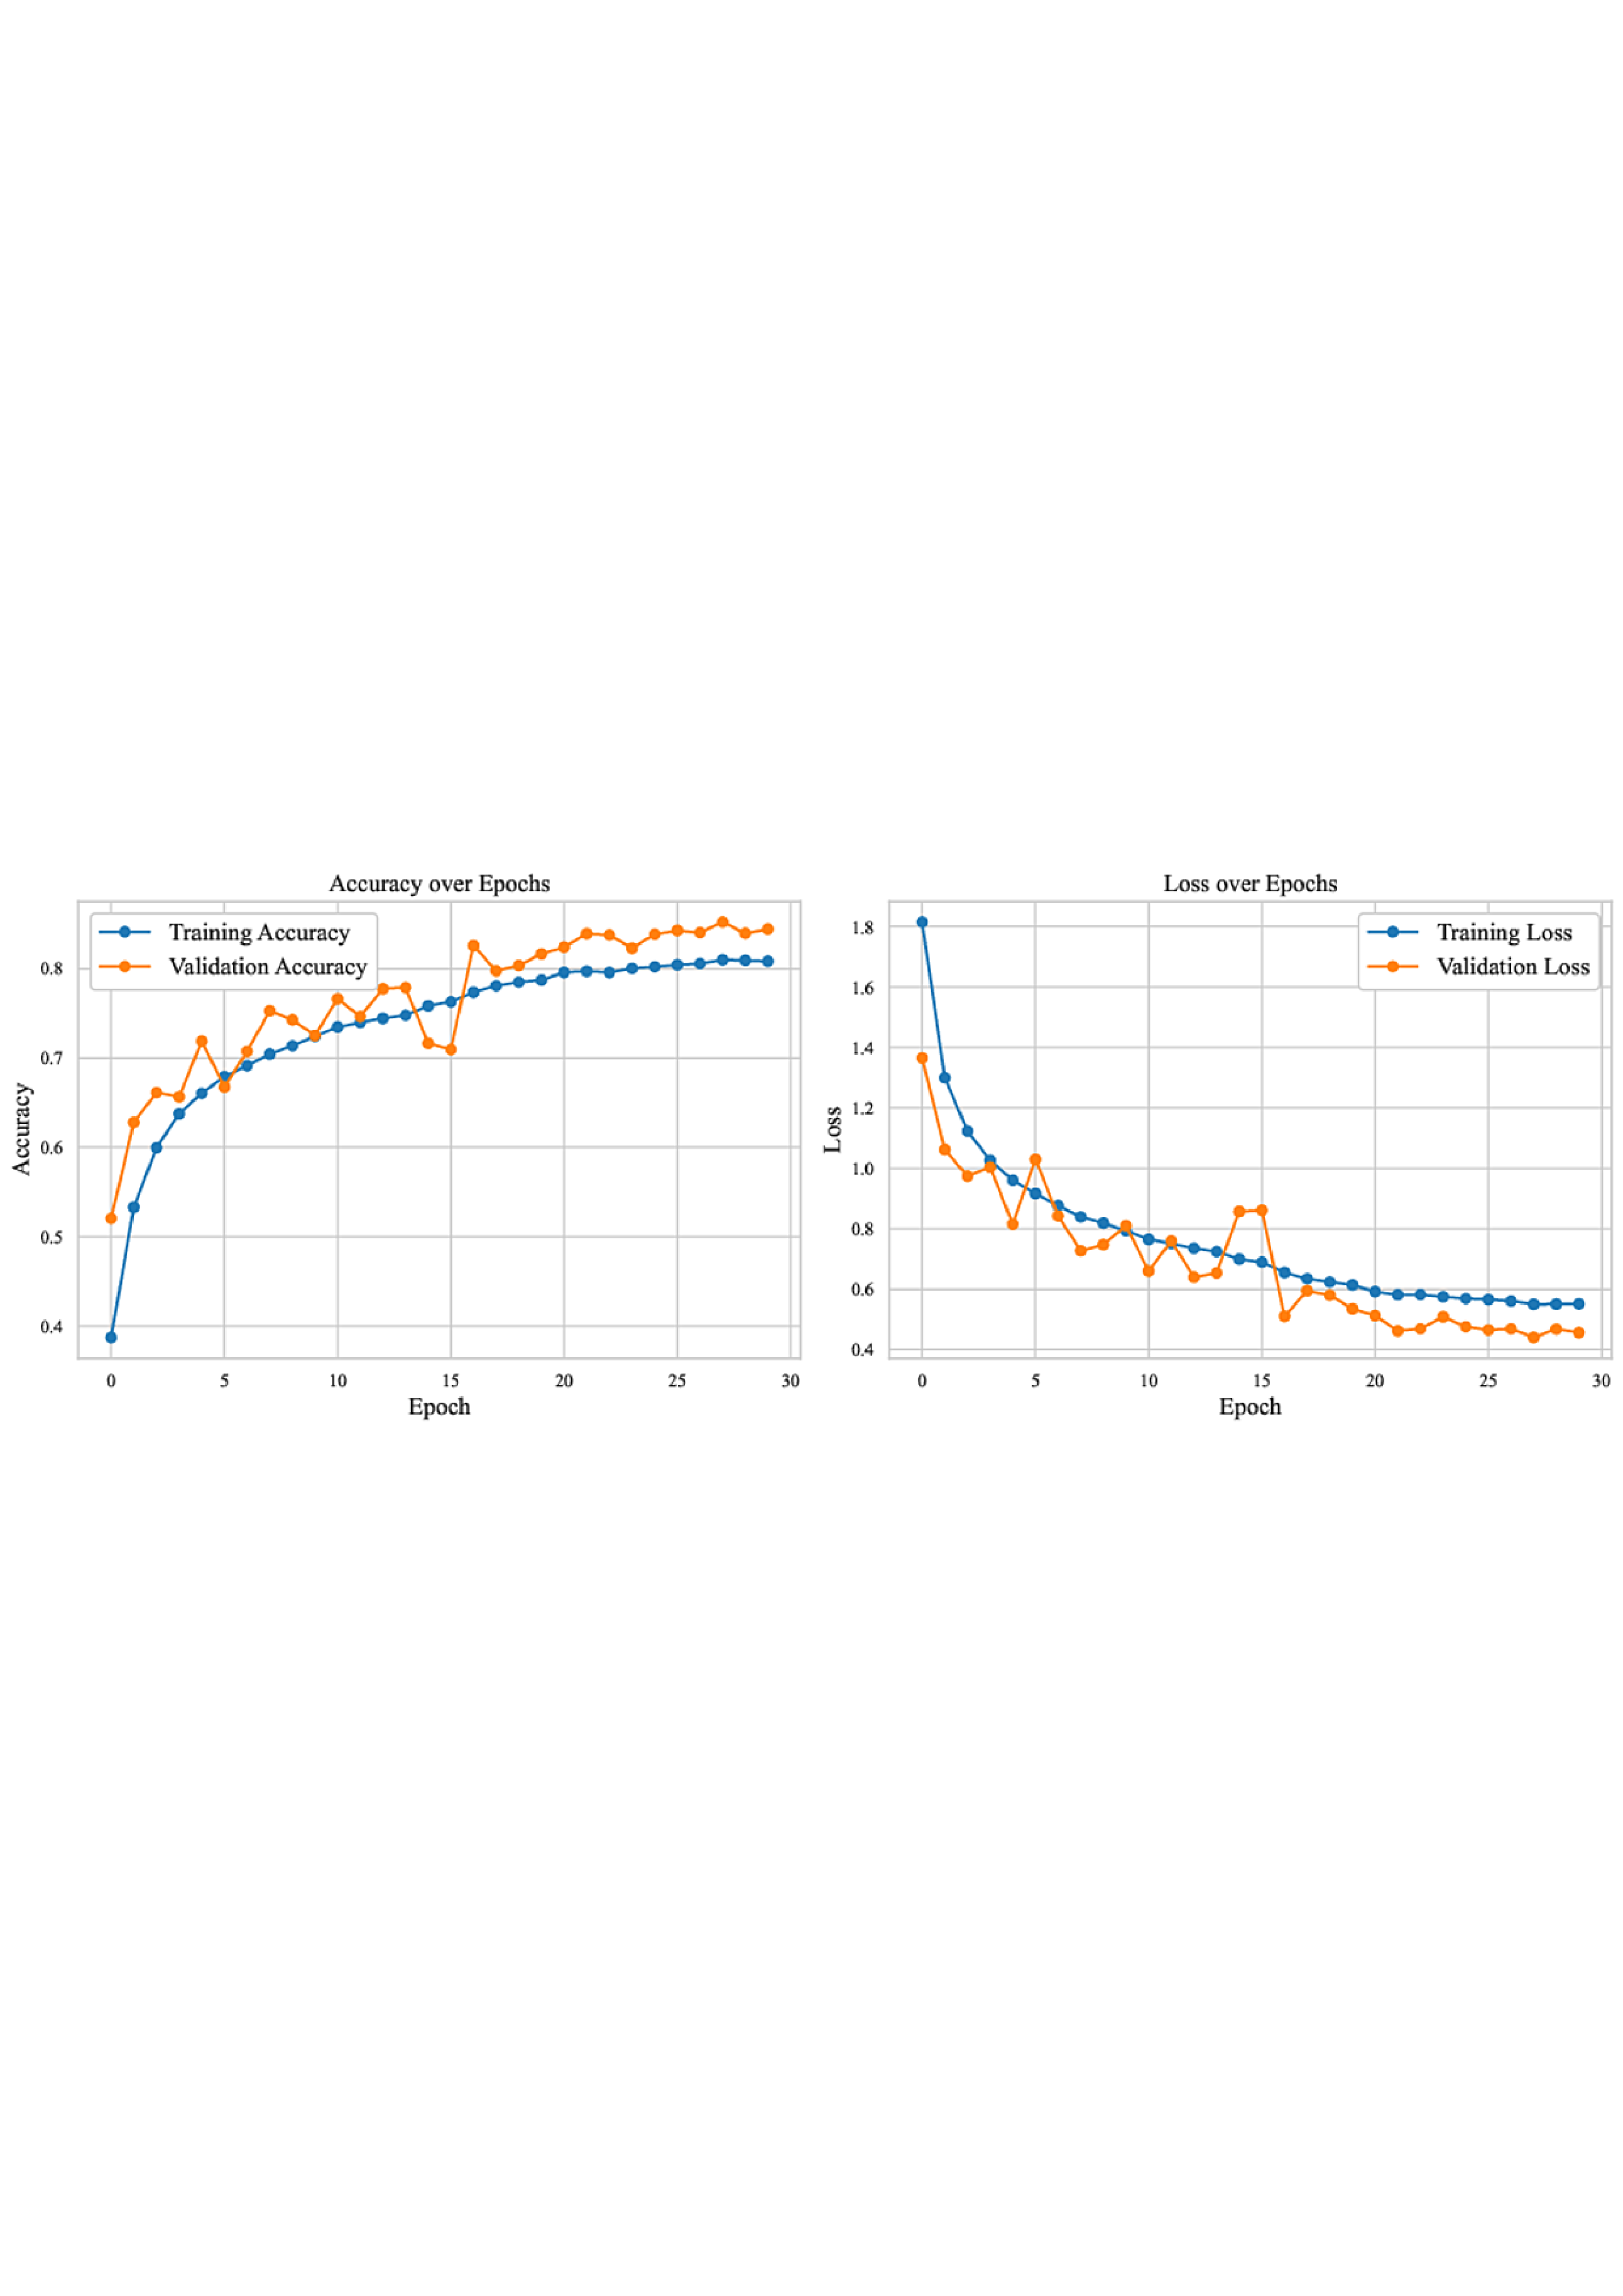
\includegraphics[width=0.9\textwidth]{training_curves.pdf}
\caption{Training and Validation Accuracy/Loss over 30 Epochs}
\end{figure}
\textbf{Observation:} Training accuracy increases steadily while validation accuracy is consistently higher and noisier - expected here, since dropout and batch normalization are active only during training, and the augmented training data is intentionally harder than the clean validation set. The validation loss curve shows visible drops each time \texttt{ReduceLROnPlateau} is implemented.

\begin{figure}[H]
\centering

\includegraphics[width=0.6\textwidth]{confusion_matrix.pdf}
\caption{Confusion Matrix on the Test Set}
\end{figure}
\textbf{Observation:} The diagonal dominates, confirming the model is right far more often than wrong, but visible off-diagonal mass sits around the cat/dog/bird block -- consistent with the per-class report showing cat's recall dragged down by the model mistaking it for other animal classes.

\begin{figure}[H]
\centering
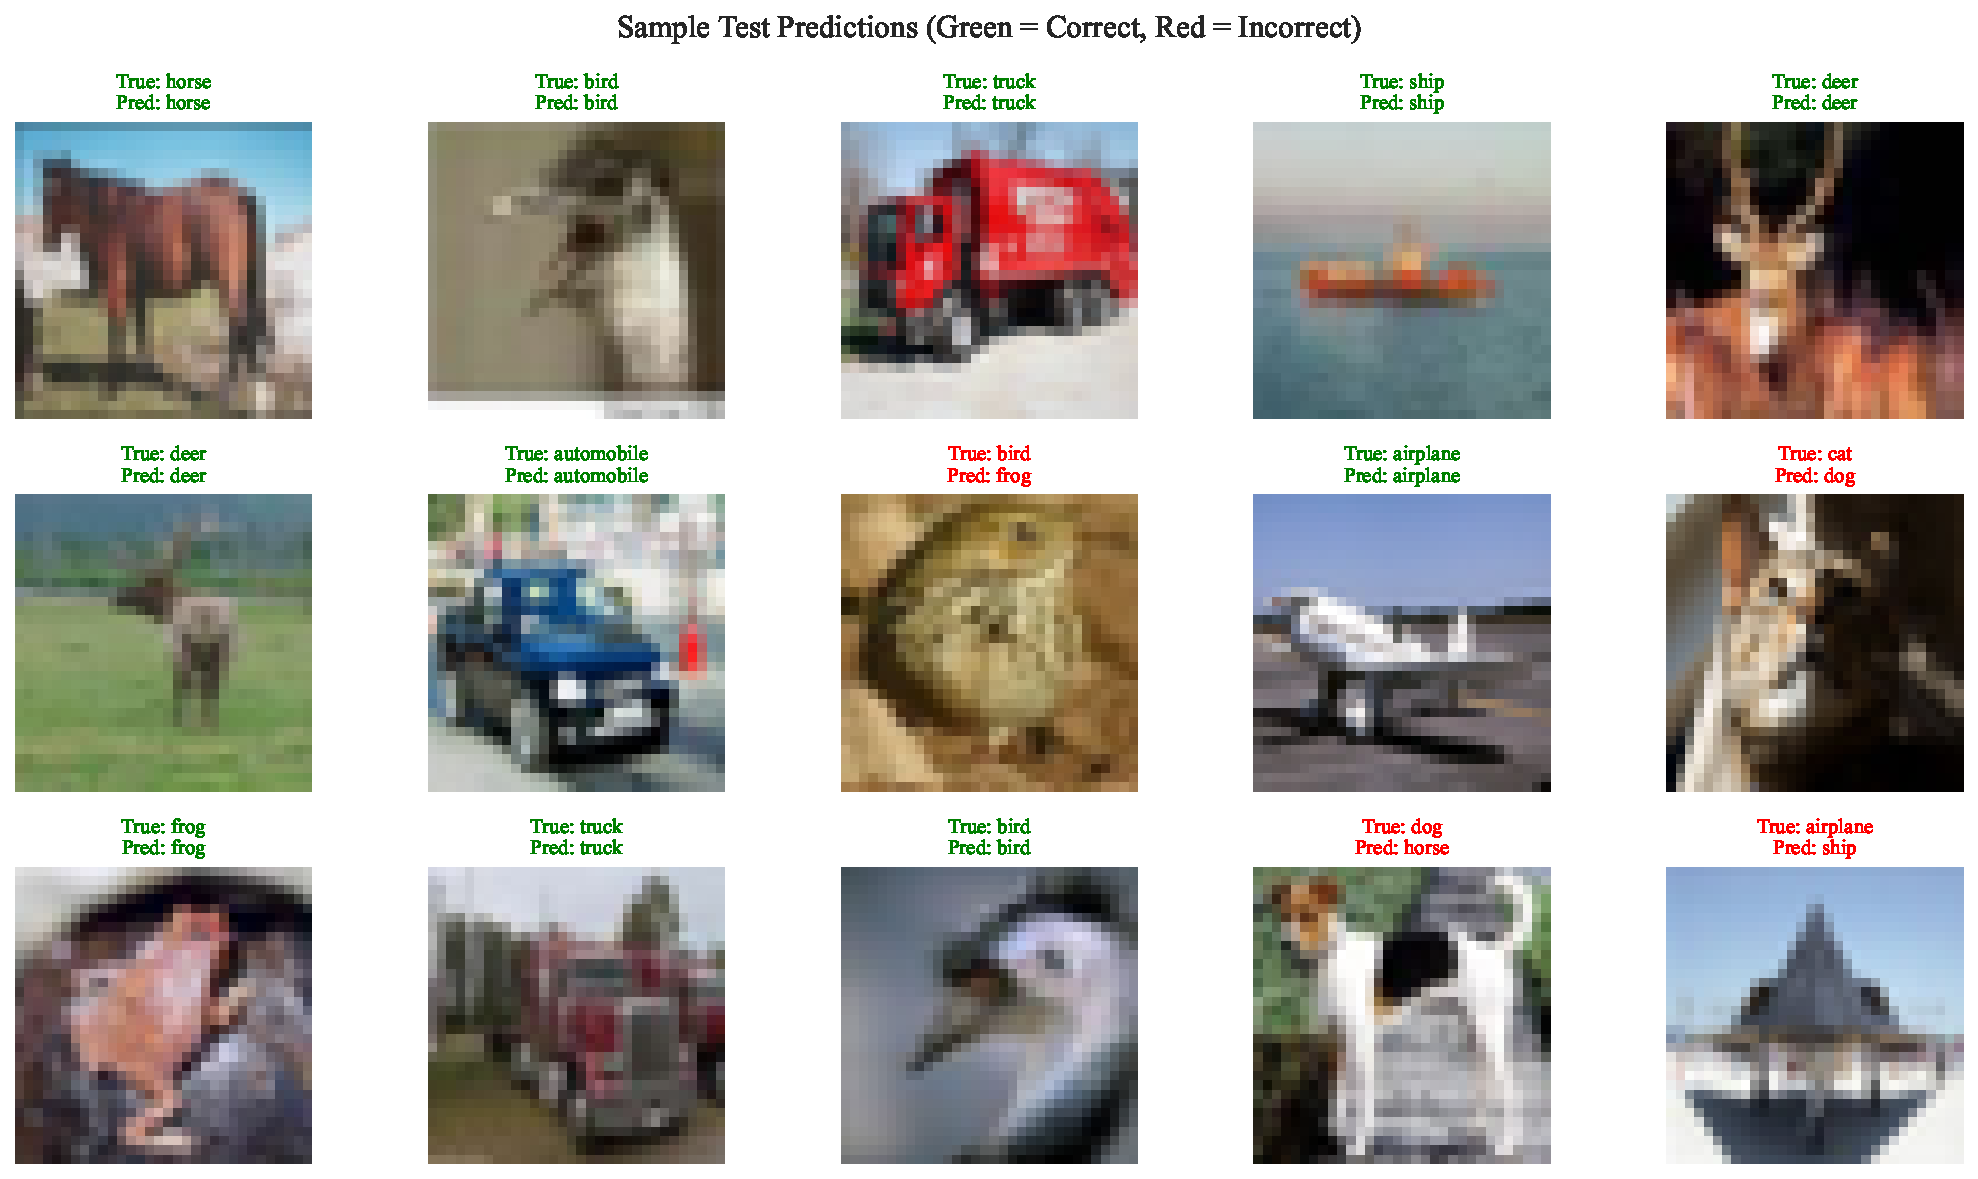
\includegraphics[width=0.85\textwidth]{sample_predictions.pdf}
\caption{Sample Test Predictions (Green = Correct, Red = Incorrect)}
\end{figure}
\textbf{Observation:} Correct predictions dominate the sample, and the visible mistakes are concentrated in exactly the classes the classification report flagged as weaker.

\begin{figure}[H]
\centering
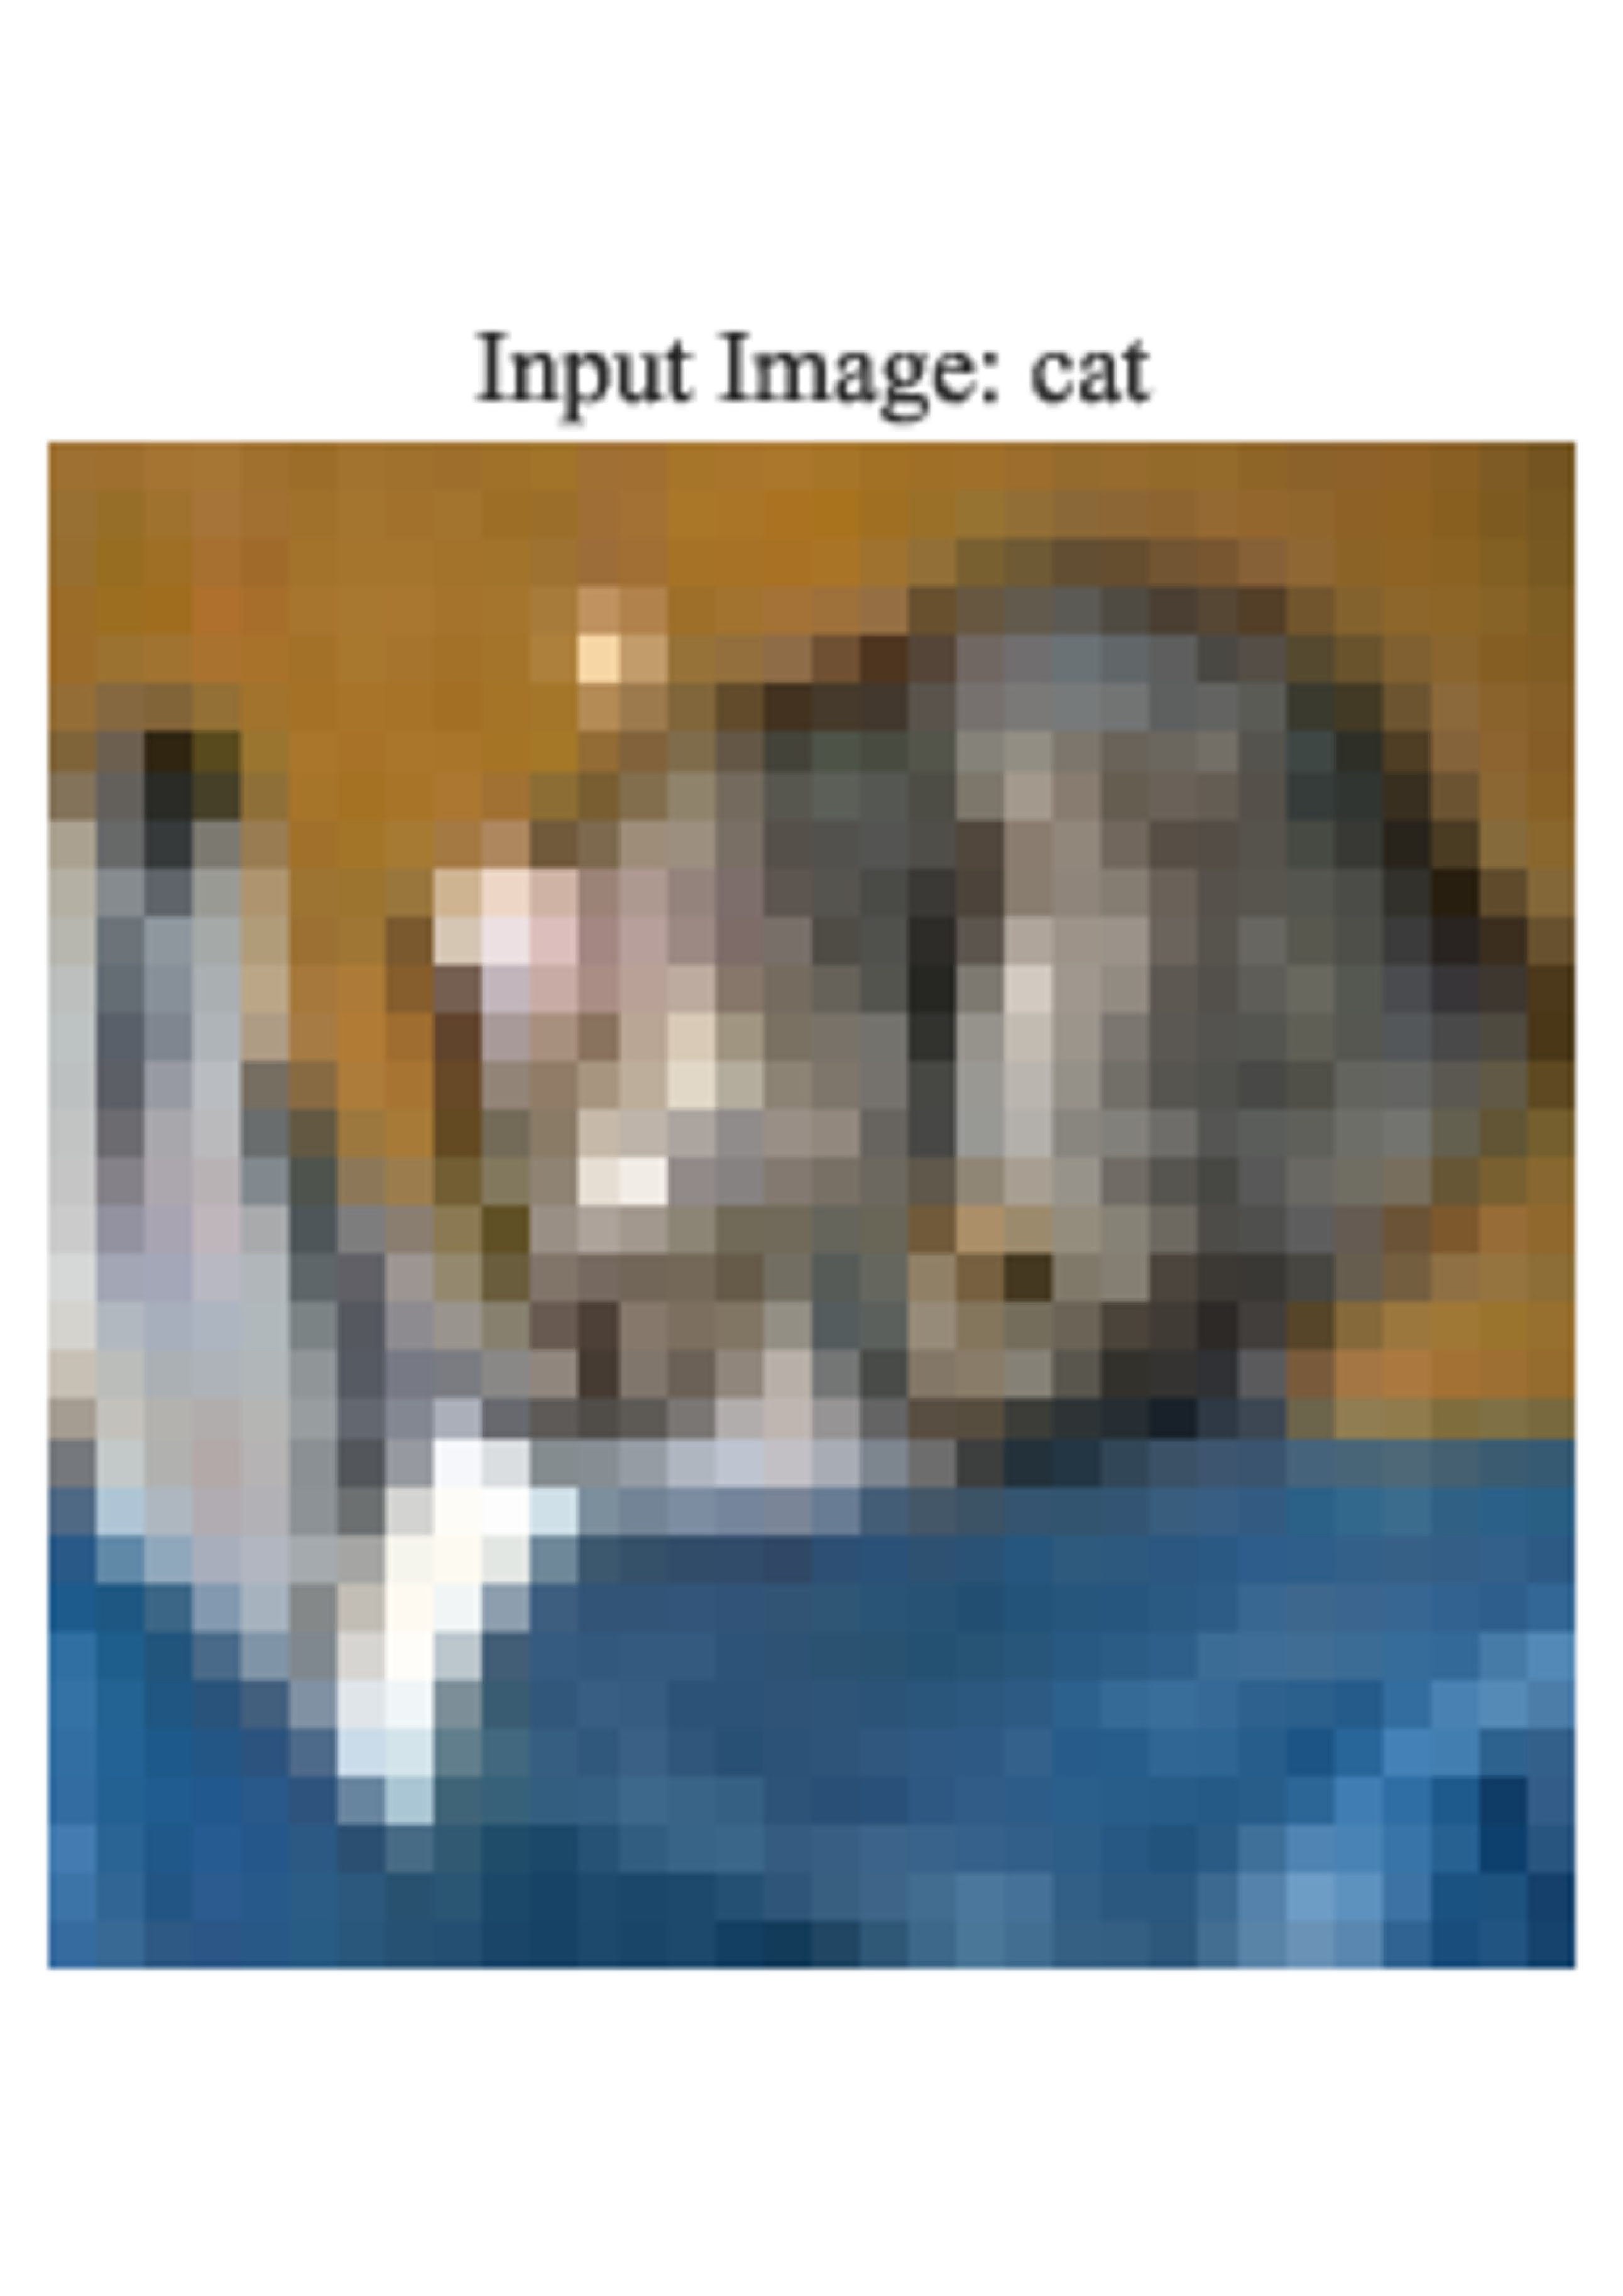
\includegraphics[width=0.35\textwidth]{feature_map_input_image.pdf}
\caption{Input Image Used for Feature Map Extraction}
\end{figure}
\textbf{Observation:} This single test image was passed through the trained network to generate every feature map shown below, so all five layers' activations can be compared against the same original picture.

\begin{figure}[H]
\centering
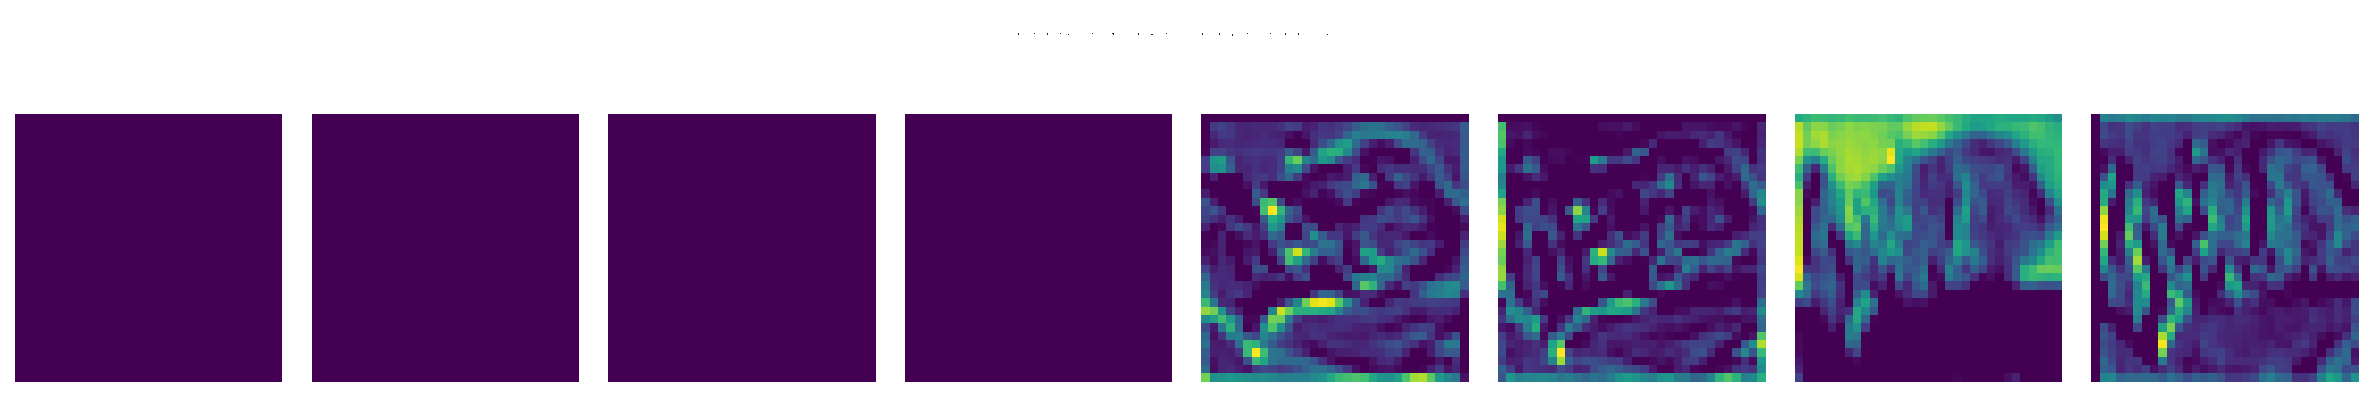
\includegraphics[width=\textwidth]{feature_maps_conv1.pdf}
\caption{Feature Maps -- Layer conv1}
\end{figure}
\textbf{Observation:} The earliest layer's feature maps closely resemble the input image itself, picking out simple edges, colour boundaries, and coarse shapes -- exactly the kind of low-level features a first convolutional layer is expected to learn. A few filters (e.g., the blank purple map) have effectively gone unused for this particular input, which is normal at this depth.

\begin{figure}[H]
\centering
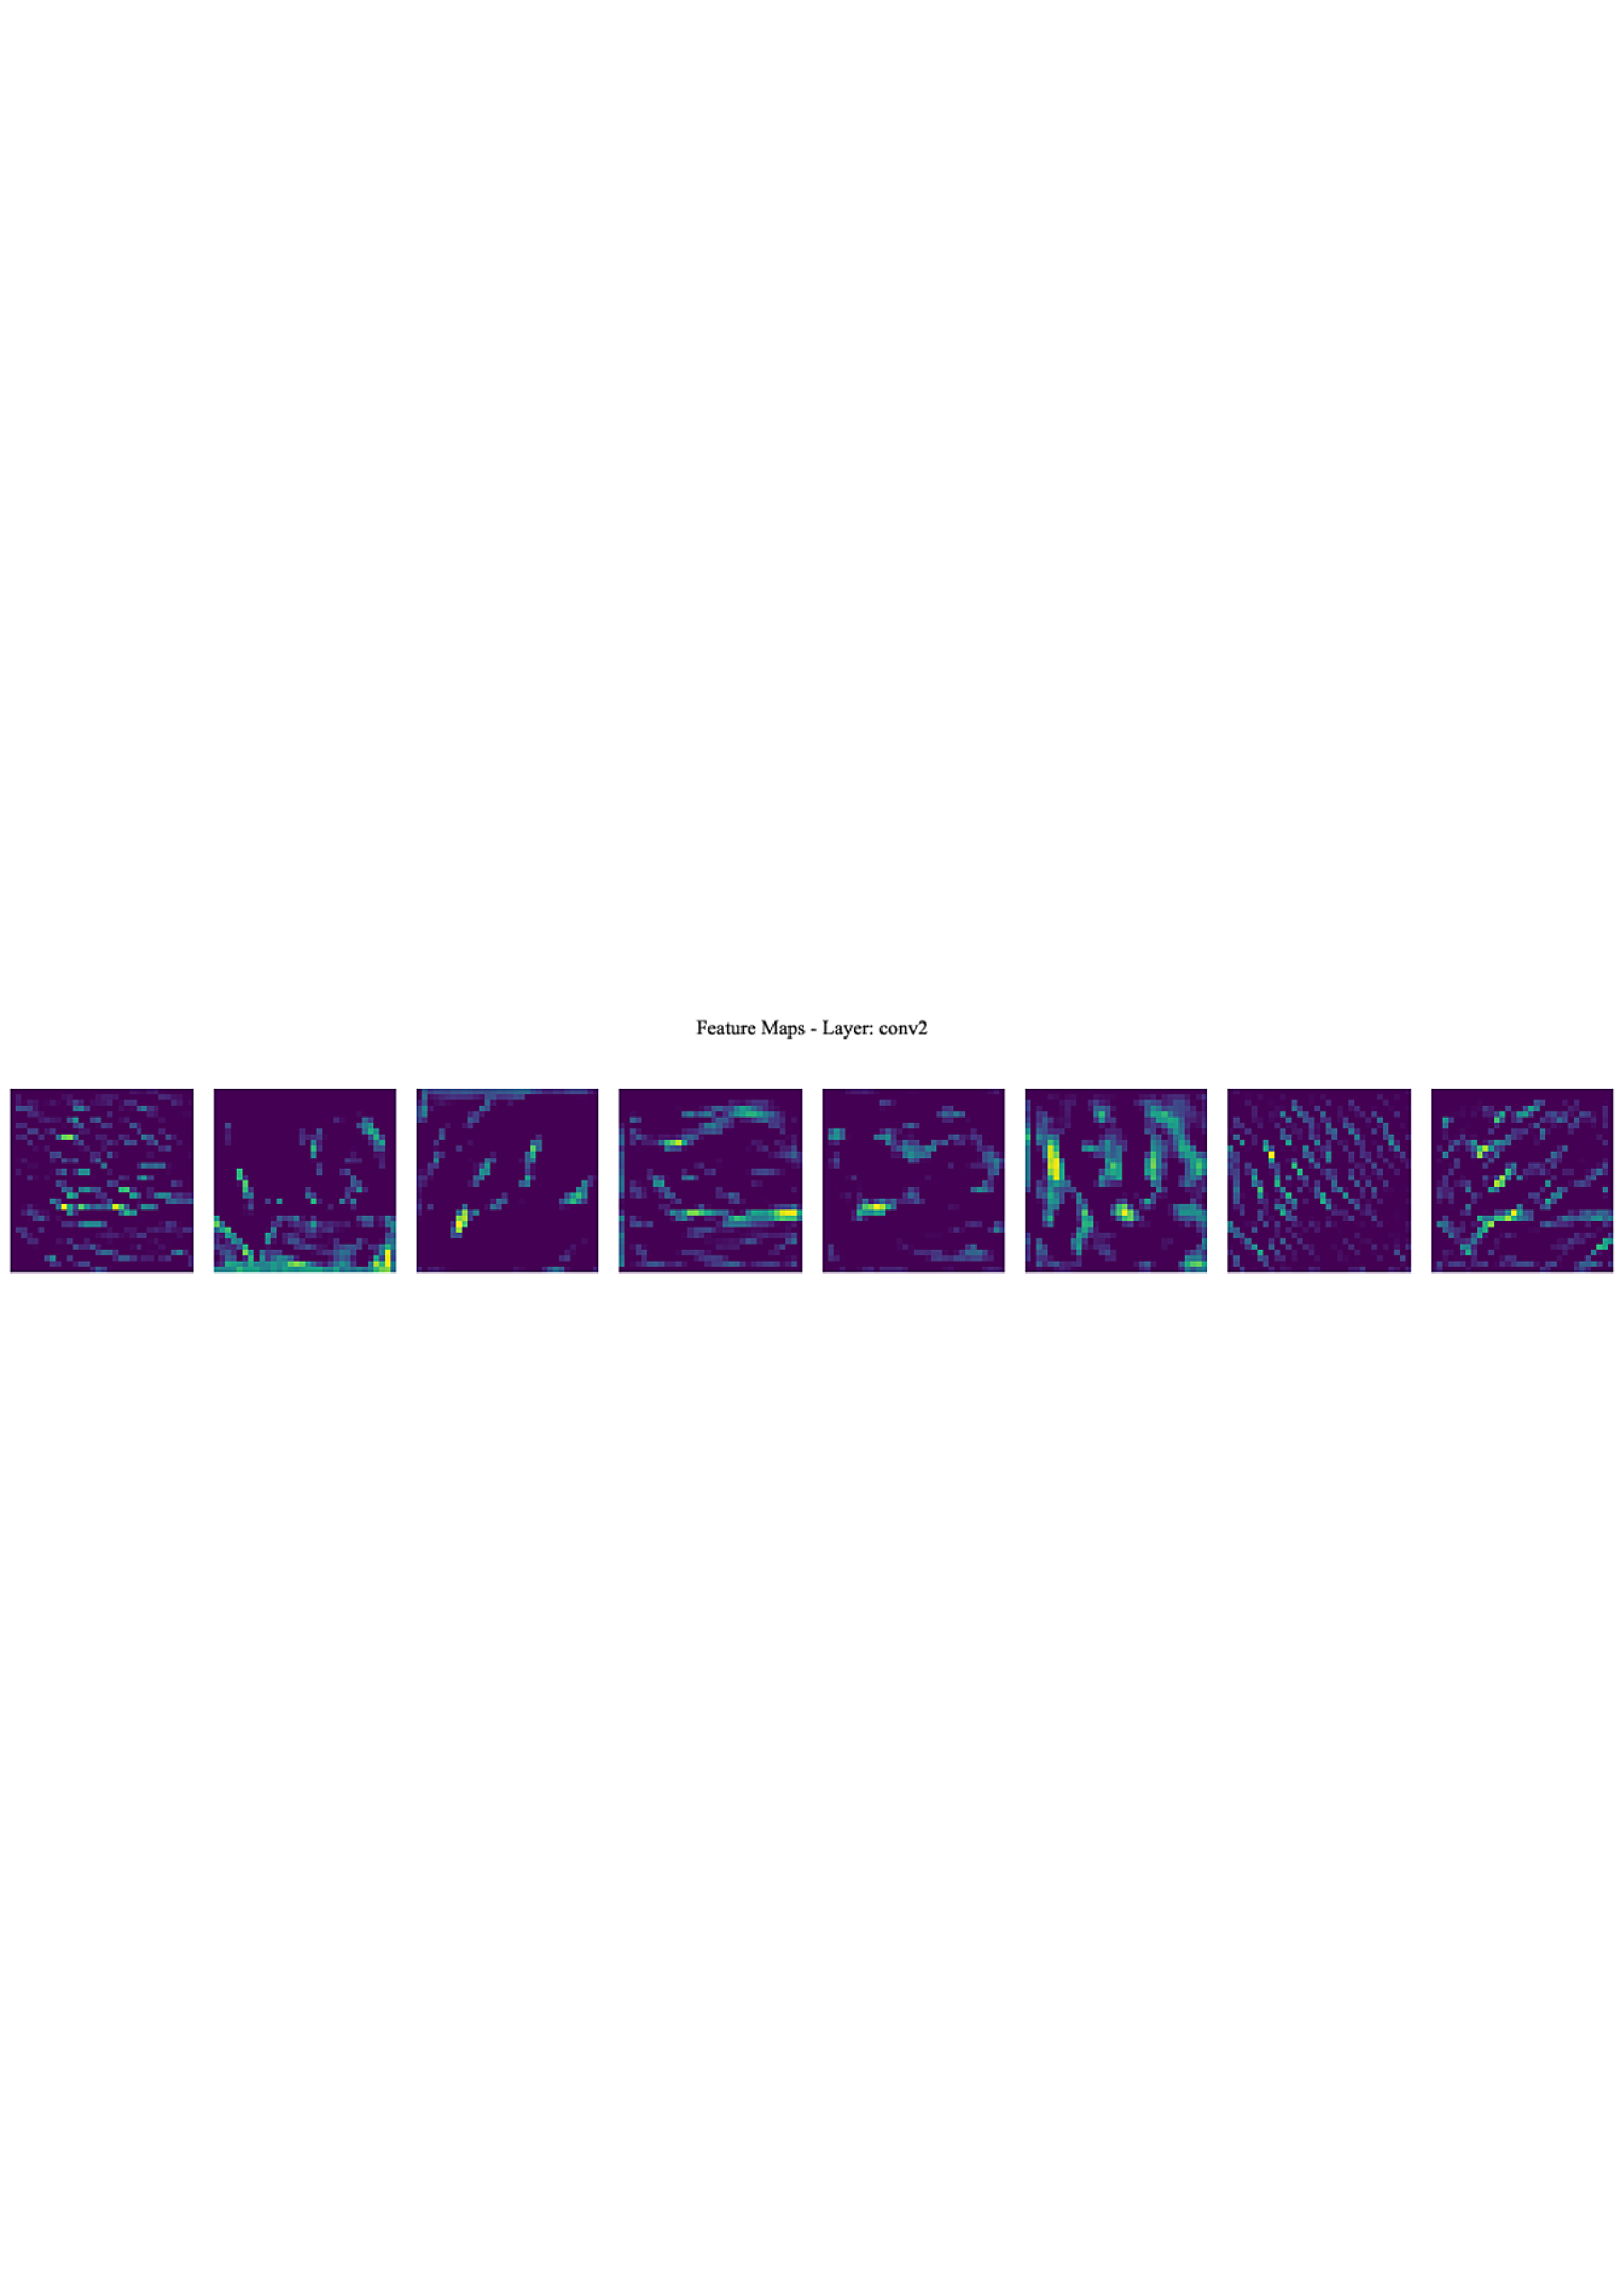
\includegraphics[width= 0.8\textwidth]{feature_maps_conv2.pdf}
\caption{Feature Maps -- Layer conv2}
\end{figure}
\textbf{Observation:} The second layer's maps are already less literal than conv1 -- the raw shape of the object is fading and being replaced by thin, directional streaks, suggesting the network is starting to respond to specific orientations and local textures rather than the whole object outline.

\begin{figure}[H]
\centering
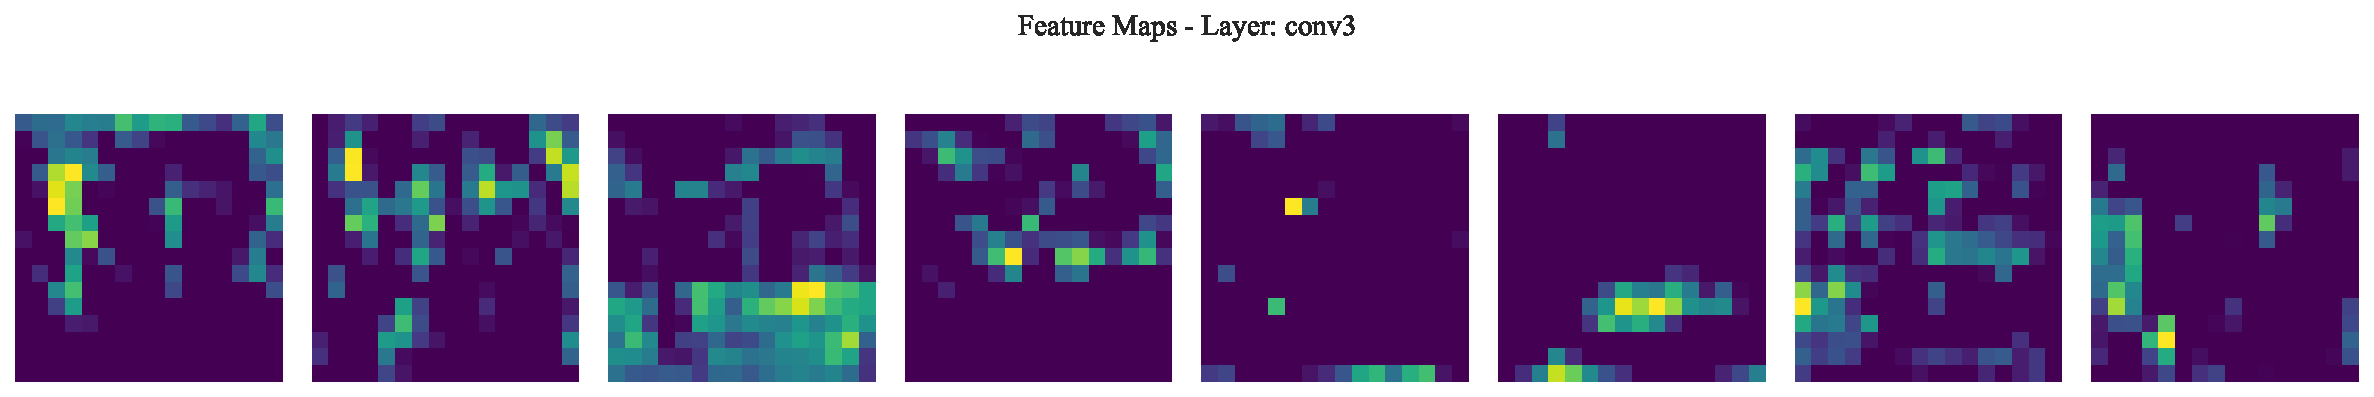
\includegraphics[width=\textwidth]{feature_maps_conv3.pdf}
\caption{Feature Maps -- Layer conv3}
\end{figure}
\textbf{Observation:} By the third convolutional layer, the feature maps are noticeably more abstract and less recognisable as the original image - the network is now combining low-level edges into more complex textures and small patterns, and the spatial resolution has also halved due to the first pooling step.

\begin{figure}[H]
\centering
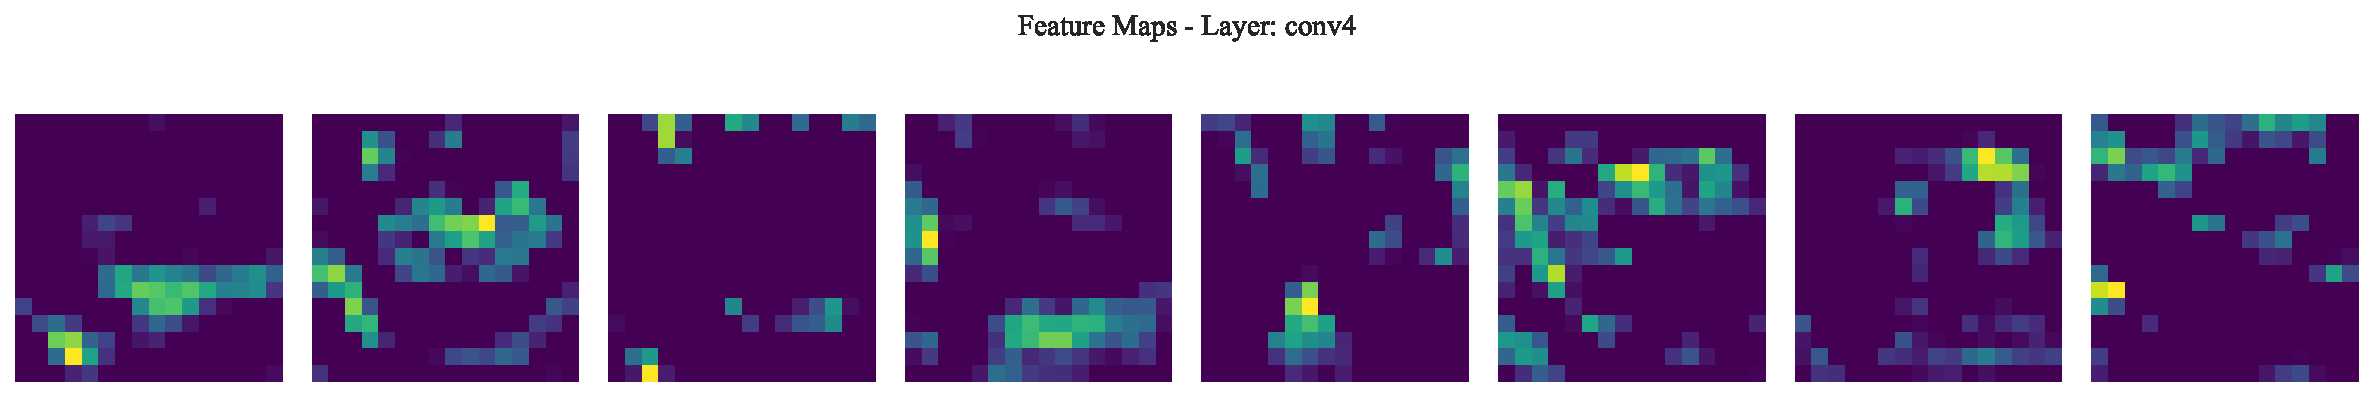
\includegraphics[width=0.85
\textwidth]{feature_maps_conv4.pdf}
\caption{Feature Maps -- Layer conv4}
\end{figure}
\textbf{Observation:} conv4's maps continue the same trend as conv3 but with sparser, more localized activations,meaning fewer pixels are firing strongly.

\begin{figure}[H]
\centering
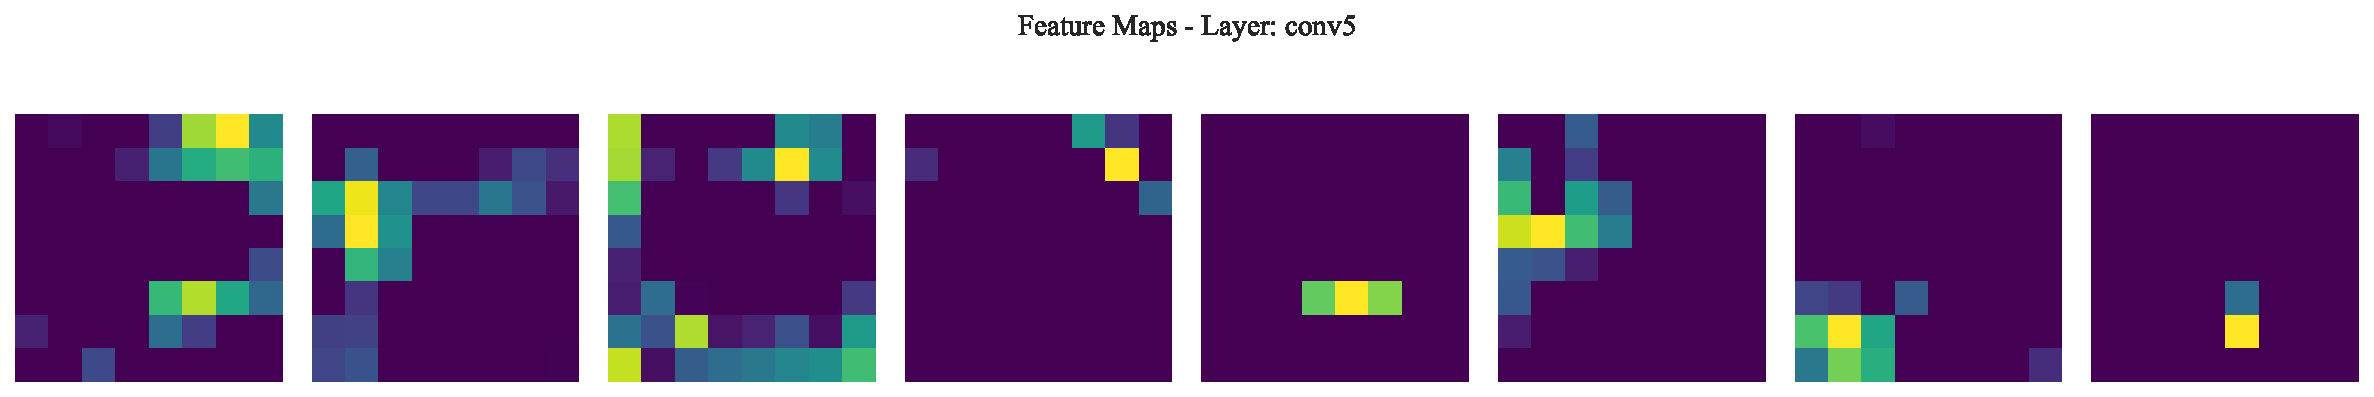
\includegraphics[width=\textwidth]{feature_maps_conv5.pdf}
\caption{Feature Maps -- Layer conv5}
\end{figure}
\textbf{Observation:} The deepest layer's feature maps are sparse and highly abstract, with only a few filters firing strongly -- this is the hierarchical feature learning behaviour CNNs are known for: early layers detect generic patterns, deep layers detect class-specific, high-level concepts.

\begin{figure}[H]
\centering
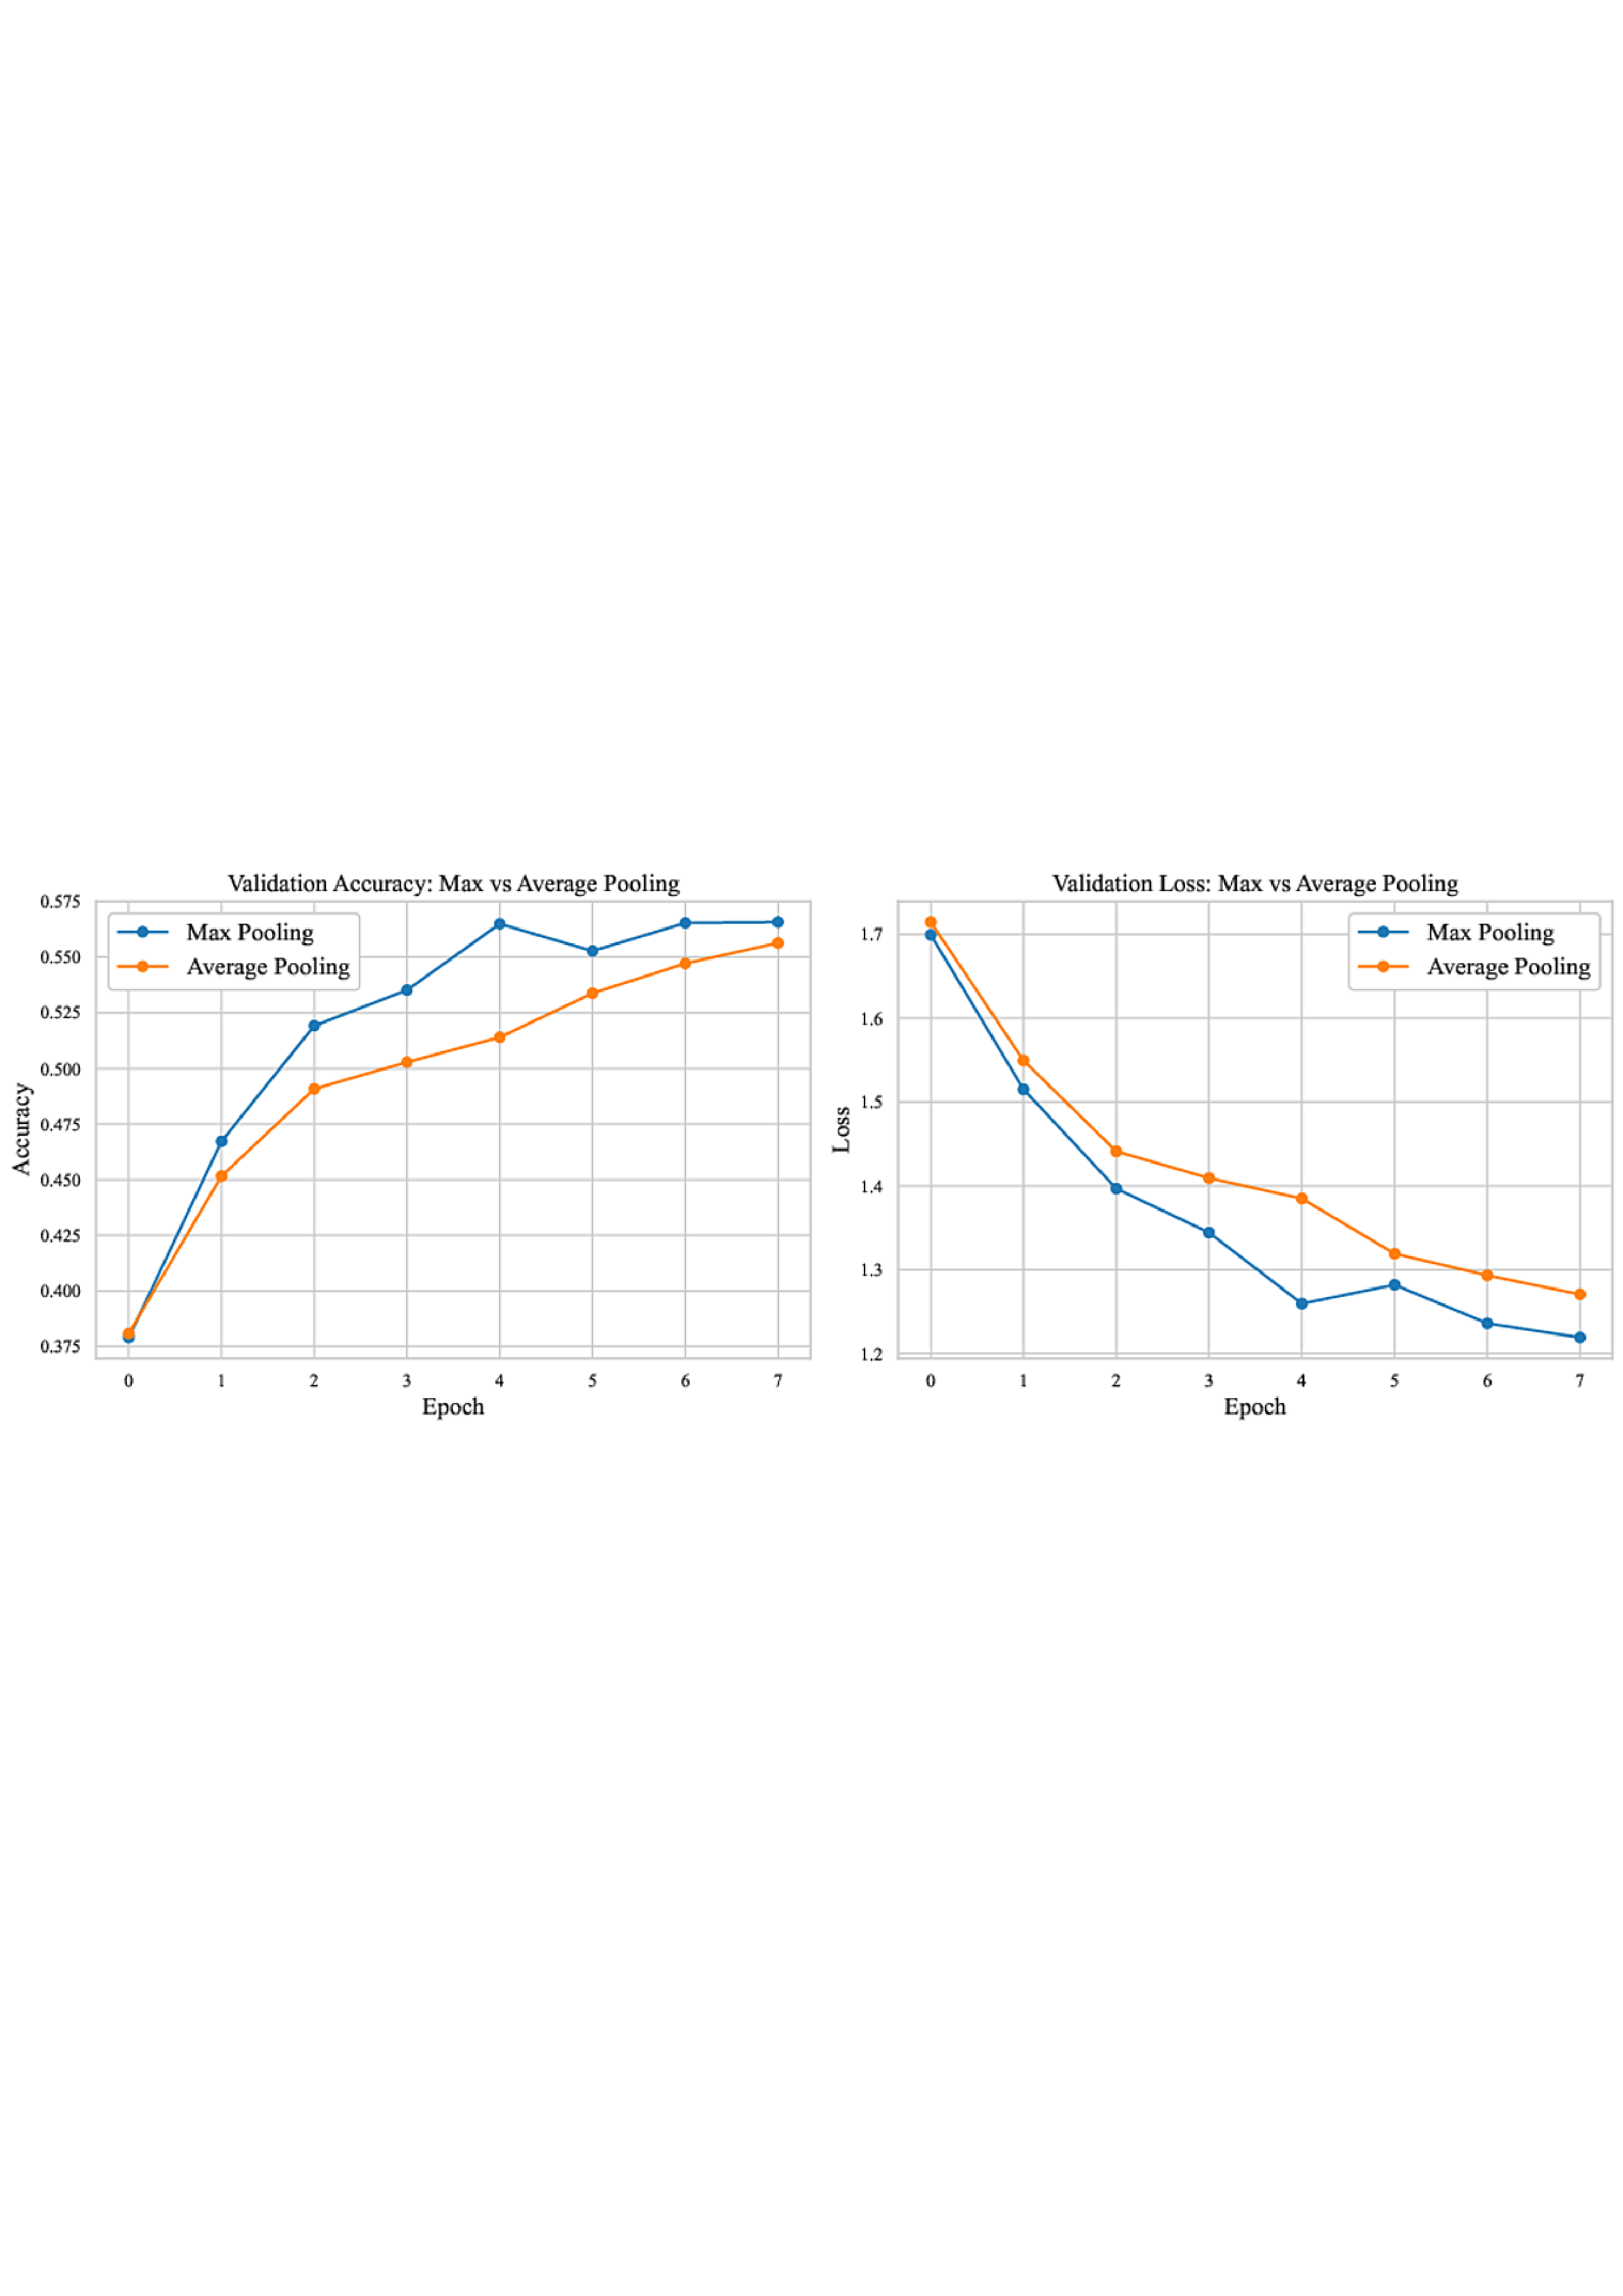
\includegraphics[width=0.8\textwidth]{pooling_comparison.pdf}
\caption{Validation Accuracy and Loss: Max vs. Average Pooling}
\end{figure}
\textbf{Observation:} The Max Pooling curve is above the Average Pooling curve for validation accuracy across all 8 epochs, matching the final test accuracy numbers in Section 7.

\begin{figure}[H]
\centering
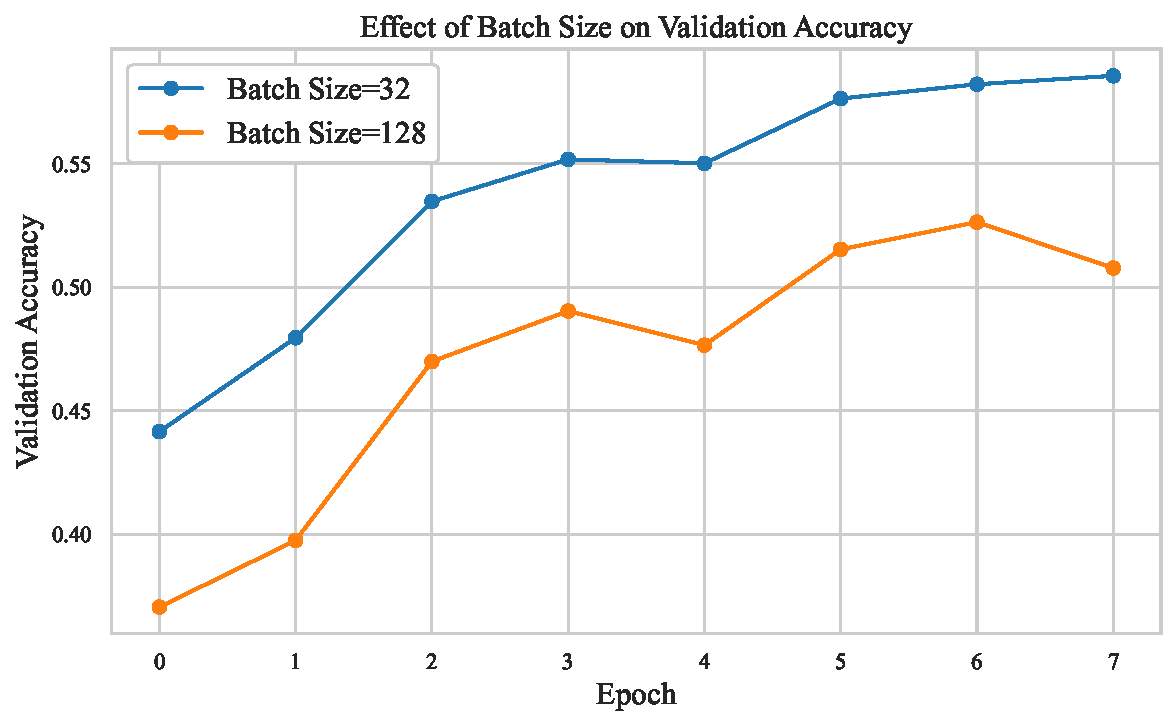
\includegraphics[width=0.6\textwidth]{batch_size_comparison.pdf}
\caption{Effect of Batch Size on Validation Accuracy}
\end{figure}
\textbf{Observation:} Batch size 32 pulls ahead of batch size 128 fairly early in training and stays ahead, reinforcing the idea that more frequent, noisier updates helped this particular short training run generalize a bit better.


%----------------------------------------------------------

\section*{9. Performance Tables}

\begin{table}[H]
\centering
\caption{Training Summary}
\begin{tabular}{ll}
\toprule
Dataset Size & 60,000 (50,000 train / 10,000 test) \\
Train/Val/Test Split & 45,000 / 5,000 / 10,000 \\
Optimizer & Adam (initial LR $=0.001$) \\
Batch Size & 64 \\
Epochs & 30 \\
LR Schedule & ReduceLROnPlateau (factor 0.5, patience 3) \\
Total Model Parameters & 668,842 \\
Test Accuracy & 0.8527 \\
Test Precision (weighted) & 0.8553 \\
Test Recall (weighted) & 0.8527 \\
Test F1-score (weighted) & 0.8501 \\
\bottomrule
\end{tabular}
\end{table}

\begin{table}[H]
\centering
\caption{Epoch-wise Training Log (Selected Epochs)}
\begin{tabular}{cccccc}
\toprule
Epoch & Train Acc. & Train Loss & Val Acc. & Val Loss & Learning Rate \\
\midrule
1  & 0.7712 & 0.6598 & 0.7958 & 0.6184 & 0.0010 \\
5  & 0.7822 & 0.6311 & 0.8272 & 0.4912 & 0.0010 \\
10 & 0.8044 & 0.5682 & 0.8516 & 0.4468 & 0.0005 \\
15 & 0.8101 & 0.5470 & 0.8442 & 0.4503 & 0.0005 \\
20 & 0.8225 & 0.5129 & 0.8492 & 0.4575 & 0.00025 \\
25 & 0.8274 & 0.4990 & 0.8684 & 0.3945 & 0.00025 \\
30 & 0.8326 & 0.4867 & 0.8482 & 0.4590 & 0.000125 \\
\bottomrule
\end{tabular}
\end{table}

%----------------------------------------------------------

\section*{10. Discussion}

This experiment offered a hands-on look at how a CNN's design choices translate into real training behaviour, beyond the theory alone. Reaching 85.27\% test accuracy on a 10-class, $32\times32$ image dataset is a solid result for an architecture of this size, and the per-class report made clear that the remaining error isn't spread evenly -- it's concentrated in a handful of visually similar animal classes.

Several observations stood out:

\begin{itemize}[leftmargin=*]
\item The learning rate schedule mattered more than expected: each of the three \texttt{ReduceLROnPlateau} drops (at epochs 9, 16, and 28) lines up with a period where validation loss had stopped improving, and training accuracy kept increasing steadily after each drop rather than stalling.
\item Cat was consistently the hardest class (recall 0.60), while frog's precision (0.74) suggests the model leans on frog as a bit of for uncertain animal predictions - a pattern that's very typical for CIFAR-10 at this scale.
\item Max Pooling outperformed Average Pooling in the short comparison, though the gap was modest (about 1 percentage point) - with more training epochs, this gap might close or widen differently, since both were evaluated on a very short 8-epoch run.
\item Batch size had a surprisingly large effect over just 8 epochs: batch 32 beat batch 128 by roughly 4.5 percentage points, telling us that smaller batches can generalize faster early in training, even if this gap wouldn't necessarily hold over a longer run.
\item The feature map visualizations gave a genuinely intuitive picture of hierarchical learning across all five convolutional layers -- conv1 looked almost like an edge-detected version of the input, the maps got progressively sparser and less literal through conv2, conv3, and conv4, and conv5 ended up as sparse, abstract activations that no longer resemble the original image at all.
\end{itemize}

%----------------------------------------------------------

\section*{11. Conclusion}

\begin{itemize}[leftmargin=*]
\item Designed and trained a 5-convolution-layer CNN (668,842 total parameters) on CIFAR-10 using TensorFlow/Keras.
\item Achieved \textbf{85.27\% test accuracy}, \textbf{85.53\% precision}, \textbf{85.27\% recall}, and an \textbf{85.01\% F1-score} on the 10,000-image held-out test set.
\item Verified the trainable parameter count of every convolutional layer, matching Keras's own count exactly.
\item Visualized feature maps across all five convolutional layers, directly observing the shift from low-level edge detection to sparse, abstract, high-level representations with depth.
\item Compared Max Pooling and Average Pooling, finding Max Pooling modestly ahead under identical short-training conditions.
\item Studied the effect of batch size, finding that a smaller batch size (32) converged to noticeably higher accuracy than a larger one (128) within the same number of epochs.
\item Identified cat, dog, and bird as the model's weakest classes, consistent with the known visual overlap between these categories in CIFAR-10.
\end{itemize}

%----------------------------------------------------------

\section*{12. References}

\begin{enumerate}
\item A. Krizhevsky, \emph{Learning Multiple Layers of Features from Tiny Images}, Technical Report, University of Toronto, 2009.
\item I. Goodfellow, Y. Bengio and A. Courville, \emph{Deep Learning}, MIT Press, 2016.
\item Y. LeCun, Y. Bengio and G. Hinton, ``Deep Learning,'' \emph{Nature}, 2015.
\item K. Simonyan and A. Zisserman, ``Very Deep Convolutional Networks for Large-Scale Image Recognition,'' \emph{ICLR}, 2015.
\item TensorFlow/Keras Documentation: Convolutional Layers and Callbacks.
\item CIFAR-10 Dataset -- University of Toronto.
\end{enumerate}

\end{document}
